\documentclass{beamer}
\usepackage{tikz,amsmath,hyperref,graphicx,stackrel,animate,media9}
\usetikzlibrary{positioning,shadows,arrows,shapes,calc}
\newcommand{\argmax}{\operatornamewithlimits{argmax}}
\newcommand{\argmin}{\operatornamewithlimits{argmin}}
\mode<presentation>{\usetheme{Frankfurt}}
\AtBeginSection[]
{
  \begin{frame}<beamer>
    \frametitle{Outline}
    \tableofcontents[currentsection,currentsubsection]
  \end{frame}
}
\title{Lecture 27: IIR Filters}
\author{Mark Hasegawa-Johnson}
\date{ECE 401: Signal and Image Analysis}  
\begin{document}

% Title
\begin{frame}
  \maketitle
\end{frame}

% Title
\begin{frame}
  \tableofcontents
\end{frame}

%%%%%%%%%%%%%%%%%%%%%%%%%%%%%%%%%%%%%%%%%%%%
\section[Review]{Review: Frequency Response}
\setcounter{subsection}{1}

\begin{frame}
  \frametitle{Review: Frequency Response}
  \begin{itemize}
  \item {\bf Tones in $\rightarrow$ Tones out}
    \begin{align*}
      x[n]=e^{j\omega n} &\rightarrow y[n]=H(\omega)e^{j\omega n}\\
      x[n]=\cos\left(\omega n\right)
      &\rightarrow y[n]=|H(\omega)|\cos\left(\omega n+\angle H(\omega)\right)\\
      x[n]=A\cos\left(\omega n+\theta\right)
      &\rightarrow y[n]=A|H(\omega)|\cos\left(\omega n+\theta+\angle H(\omega)\right)
    \end{align*}
  \item where the {\bf Frequency Response} is given by
    \[
    H(\omega) = \sum_m h[m]e^{-j\omega m}
    \]
  \end{itemize}
\end{frame}  

\begin{frame}
  \frametitle{Example: First Difference}

  \begin{displaymath}
    y[n] = x[n]-x[n-1] = \sum_m h[m] x[n-m]
  \end{displaymath}
  \begin{displaymath}
    h[n] =\begin{cases}
    1 & n=0\\
    -1 & n=1\\
    0&\mbox{otherwise}
    \end{cases}
  \end{displaymath}
  \begin{displaymath}
    H(\omega) = \sum_m h[m]e^{-j\omega m} = 1-e^{-j\omega}
  \end{displaymath}
\end{frame}

\begin{frame}
  \frametitle{Another way to think about first difference}

  \begin{equation}
    y[n] = x[n]-x[n-1]
    \label{eq:diff}
  \end{equation}
  But remember the delay property of the DTFT:
  \begin{displaymath}
    x[n-k] \leftrightarrow e^{-j\omega k}X(\omega)
  \end{displaymath}
  So we could take the DTFT of each term in Eq.~(\ref{eq:diff}) to
  get:
  \begin{displaymath}
    Y(\omega) = X(\omega) - e^{-j\omega}X(\omega) = \left(1-e^{-j\omega}\right)X(\omega)
  \end{displaymath}
\end{frame}

\begin{frame}
  \frametitle{Another way to think about first difference}

  \begin{displaymath}
    Y(\omega) = X(\omega) - e^{-j\omega}X(\omega) = \left(1-e^{-j\omega}\right)X(\omega)
  \end{displaymath}
  But remember the convolution property of the DTFT:
  \begin{displaymath}
    y[n]=h[n]\ast x[n] \leftrightarrow Y(\omega) = H(\omega)X(\omega)
  \end{displaymath}
  So we find that:
  \begin{displaymath}
    H(\omega)=\frac{Y(\omega)}{X(\omega)} = 1-e^{-j\omega}
  \end{displaymath}
\end{frame}

%%%%%%%%%%%%%%%%%%%%%%%%%%%%%%%%%%%%%%%%%%%%
\section[Autoregressive]{Autoregressive Difference Equations}
\setcounter{subsection}{1}

\begin{frame}
  \frametitle{Autoregressive Filter}

  Today, instead of filters with this form:
  \begin{displaymath}
    y[n] = x[n]-x[n-1]
  \end{displaymath}
  \ldots we want to start studying filters of this form:
  \begin{displaymath}
    y[n] = x[n]-y[n-1]
  \end{displaymath}
  \begin{itemize}
  \item This is called {\bf autoregressive}, meaning that $y[n]$ depends on
    past values (regressive) of itself (auto).
  \item This is also an {\bf infinite impulse response} (IIR) filter, because
    the impulse response ($h[n]$) is infinitely long.
  \end{itemize}
\end{frame}
    
\begin{frame}
  \frametitle{Autoregressive Difference Equations}

  An {\bf autoregressive} filter is one in which the output, $y[n]$,
  depends on past values of itself ({\bf auto}=self, {\bf
    regress}=go back).  For example,
  \[
  y[n] = x[n] + 0.3x[n-1] + 0.8 y[n-1]
  \]
  
\end{frame}

\begin{frame}
  \frametitle{Causal and Anti-Causal Filters}

  \begin{itemize}
  \item If the outputs of a filter depend only on {\bf current and
    past} values of the input, then the filter is said to be {\bf
    causal}.  An example is
    \[
    y[n] = x[n] + 0.3x[n-1] + 0.8 y[n-1]
    \]
  \item If the outputs depend only on {\bf current and future} values
    of the input, the filter is said to be {\bf anti-causal}, for example
    \[
    y[n]=x[n]+0.3x[n+1]+0.8y[n+1]
    \]
  \item If the filter is neither causal nor anti-causal, we say it's
    ``non-causal.''
  \item Feedforward non-causal filters are easy to analyze, but when
    analyzing feedback, we will stick to causal filters.
  \end{itemize}
  
\end{frame}

\begin{frame}
  \frametitle{Autoregressive Difference Equations}

  We can find the frequency response by taking the DTFT of each term
  in the equation:
  \begin{align*}
    y[n] &= x[n] + 0.3 x[n-1] +  0.8 y[n-1]\\
    Y(\omega) &= X(\omega) + 0.3e^{-j\omega}X(\omega) + 0.8  e^{-j\omega}Y(z)
  \end{align*}
  
\end{frame}

\begin{frame}
  \frametitle{Frequency Response}

  In order to find the frequency response, we need to solve for
  $H(\omega)=\frac{Y(\omega)}{X(\omega)}$.
  \begin{align*}
    Y(\omega) &= X(\omega) + 0.3e^{-j\omega}X(\omega) + 0.8 e^{-j\omega}Y(\omega)\\
    \left(1-0.8e^{-j\omega}\right)Y(\omega) &= X(\omega)(1+0.3e^{-j\omega})\\
    H(\omega) =\frac{Y(\omega)}{X(\omega)} &= \frac{1+0.3e^{-j\omega}}{1-0.8 e^{-j\omega}}
  \end{align*}
\end{frame}

\begin{frame}
  \frametitle{Frequency Response}

  Here is the frequency response of this filter, plotted using {\tt
    np.abs((1+0.3*np.exp(-1j*omega))/(1-0.8*np.exp(-1j*omega)))}
  
  \centerline{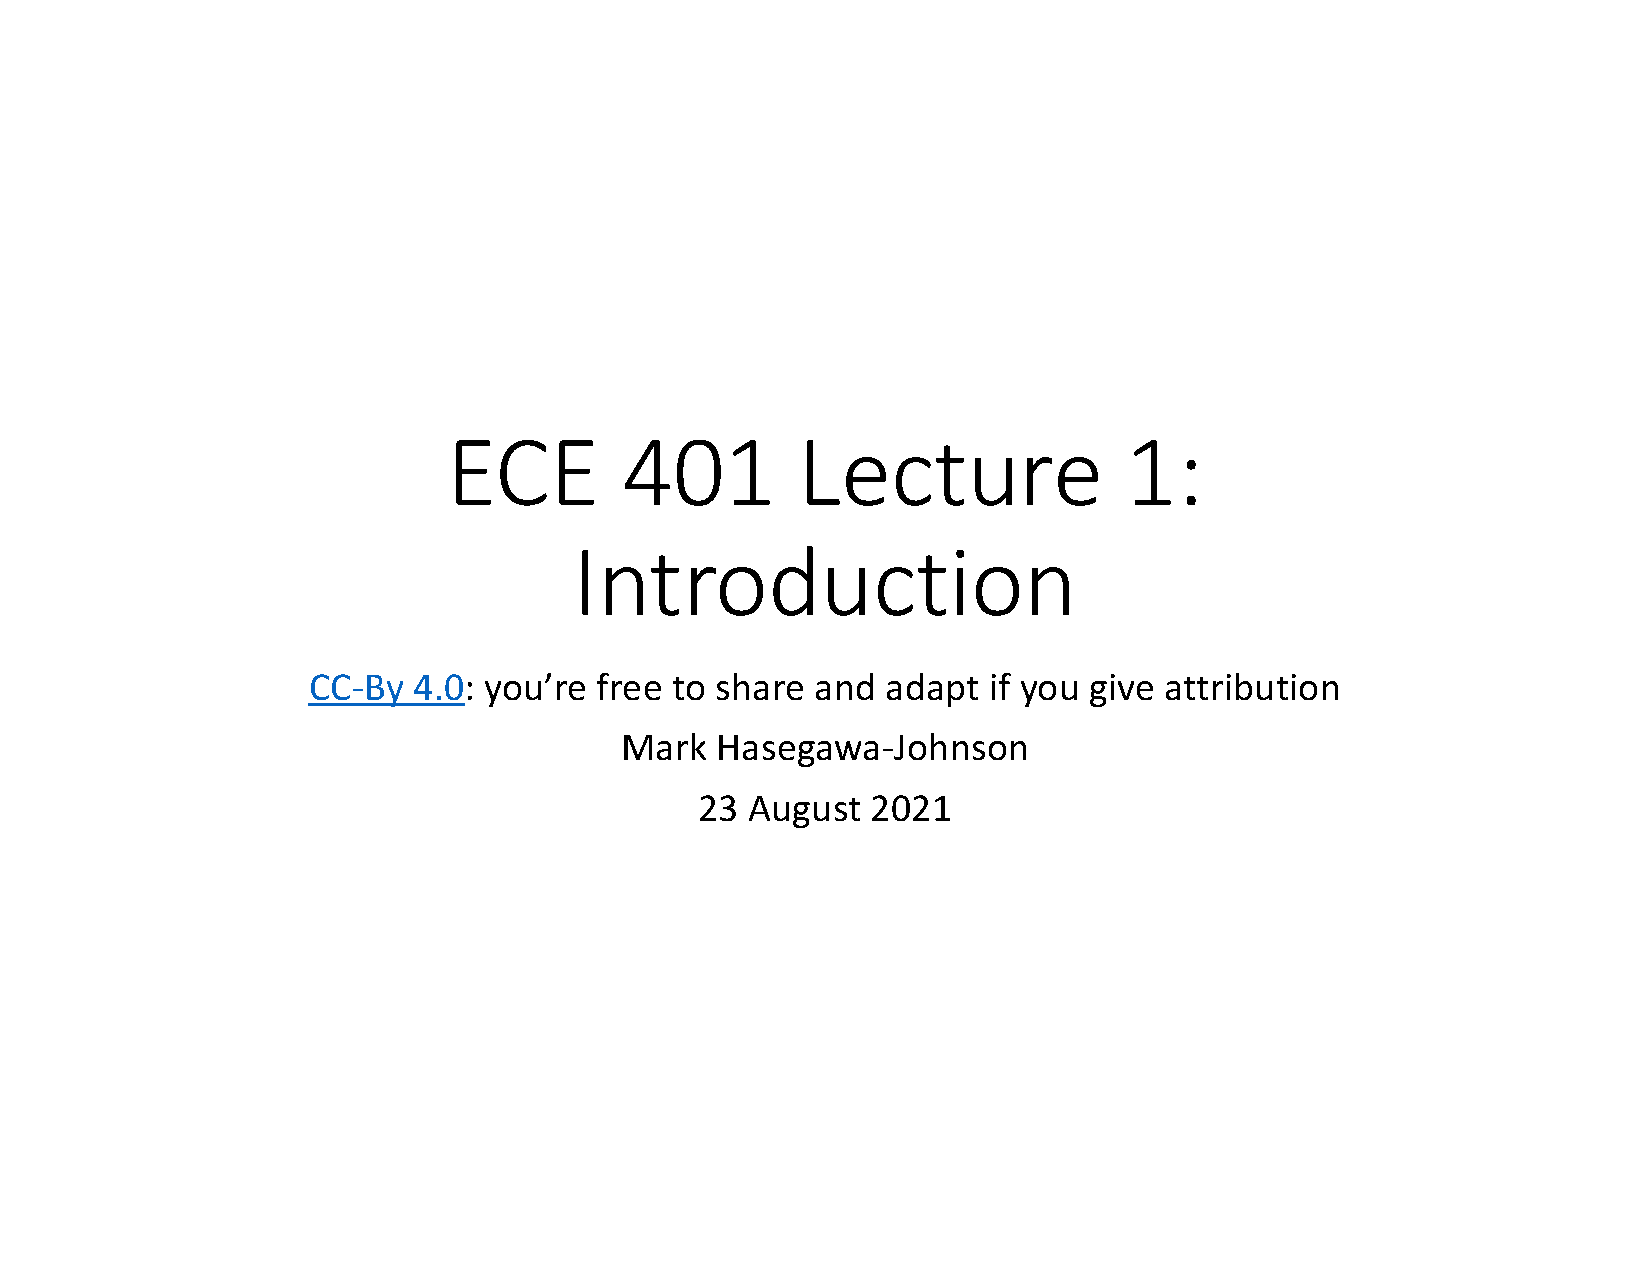
\includegraphics[height=2.5in]{exp/intro.png}}
\end{frame}

%%%%%%%%%%%%%%%%%%%%%%%%%%%%%%%%%%%%%%%%%%%%
\section[FIR and IIR]{Finite vs. Infinite Impulse Response}
\setcounter{subsection}{1}

\begin{frame}
  \frametitle{Impulse Response of an Autoregressive Filter}

  One way to find the {\bf impulse response} of an autoregressive
  filter is the same as for any other filter: feed in an impulse,
  $x[n]=\delta[n]$, and what comes out is the impulse response,
  $y[n]=h[n]$.
  \[
  h[n] = \delta[n] + 0.3\delta[n-1] + 0.8 h[n-1]
  \]
  %Because it's autoregressive, we have to solve for $h[n]$ recursively:
  \begin{align*}
    h[n] &= 0,~~n<0\\
    h[0] &= \delta[0] = 1\\
    h[1] &= 0 + 0.3\delta[0] + 0.8 h[0] = 1.1\\
    h[2] &= 0 + 0 + 0.8 h[1] = 0.88\\
    h[3] &= 0+ 0 + 0.8 h[2] = 0.704\\
    & \vdots\\
    h[n] &= 1.1(0.8)^{n-1}~~\mbox{if}~n\ge 1\\
    & \vdots\\
  \end{align*}
\end{frame}

\begin{frame}
  \frametitle{FIR vs. IIR Filters}

  \begin{itemize}
  \item Most autoregressive filters are also {\bf infinite
    impulse response (IIR)} filters, because $h[n]$ is infinitely long
    (never ends).
  \item A difference equation with only feedforward terms (like we saw
    in the last lecture) is always a {\bf finite impulse response
      (FIR)} filter, because $h[n]$ has finite length.
  \end{itemize}
\end{frame}

\begin{frame}
  \frametitle{General form of an FIR filter}
  \begin{align*}
    y[n] &= \sum_{k=0}^{M} b_k x[n-k] = \sum_k h[k]x[n-k]\\
    h[k] &=\begin{cases}
    b_k & 0\le k\le M\\
    0 &\mbox{otherwise}
    \end{cases}
  \end{align*}
  This filter has an impulse response ($h[n]$) that is $M+1$ samples
  long.
  \begin{itemize}
  \item The $b_k$'s are called {\bf feedforward}
    coefficients, because they feed $x[n]$ forward into $y[n]$.
  \end{itemize}
\end{frame}

\begin{frame}
  \frametitle{General form of an IIR filter}
  \[
  \sum_{\ell=0}^N a_\ell y[n-\ell] = \sum_{k=0}^{M} b_k x[n-k]
  \]
  \begin{itemize}
  \item %The general form of an IIR filter is $\sum_{\ell=0}^N a_\ell
    %y[n-\ell] = \sum_{k=0}^{M} b_k x[n-k]$.
    The $a_\ell$'s are caled
    {\bf feedback} coefficients, because they feed $y[n]$ back into
    itself.
    %The impulse response is infinite length.  In order to
    %find its general form, we need a bit more math.
  \item Can we find $h[n]$ in terms of $a_\ell$ and $b_k$?
  \end{itemize}
\end{frame}

%%%%%%%%%%%%%%%%%%%%%%%%%%%%%%%%%%%%%%%%%%%%
\section[First-Order]{Impulse Response and Transfer Function of a First-Order Autoregressive Filter}
\setcounter{subsection}{1}

\begin{frame}
  \frametitle{First-Order Feedback-Only Filter}

  Let's find the general form of $h[n]$, for the simplest possible
  autoregressive filter: a filter with one feedback term, and no
  feedforward terms, like this:
  \[
  y[n] = x[n] + ay[n-1],
  \]
  where $a$ is any constant (positive, negative, real, or complex).
\end{frame}

\begin{frame}
  \frametitle{Impulse Response of a First-Order Filter}

  We can find the impulse response by putting in $x[n]=\delta[n]$, and
  getting out $y[n]=h[n]$:
  \[
  h[n] = \delta[n] + ah[n-1].
  \]
  Recursive computation gives
  \begin{align*}
    h[0] &= 1 \\
    h[1] &= a\\
    h[2] &= a^2\\
     & \vdots\\
    h[n] &= a^nu[n]
  \end{align*}
  where we use the notation $u[n]$ to mean the ``unit step function,''
  \[u[n] = \begin{cases}1& n\ge 0\\0 & n<0\end{cases}\]
\end{frame}

\begin{frame}
  \frametitle{Impulse Response of Stable First-Order Filters}

  The coefficient, $a$, can be positive, negative, or even complex.
  If $a$ is complex, then $h[n]$ is also complex-valued.
  \centerline{\includegraphics[height=2.5in]{exp/iir_stable.png}}

\end{frame}

\begin{frame}
  \frametitle{Impulse Response of Unstable First-Order Filters}

  If $|a|>1$, then the impulse response grows exponentially.  If
  $|a|=1$, then the impulse response never dies away.  In either case,
  we say the filter is ``unstable.''
  \centerline{\includegraphics[height=2.5in]{exp/iir_unstable.png}}

\end{frame}

\begin{frame}
  \frametitle{Instability}

  \begin{itemize}
  \item A {\bf stable} filter is one that always generates finite
    outputs ($|y[n]|$ finite) for every possible finite input
    ($|x[n]|$ finite).
  \item An {\bf unstable} filter is one that, at least sometimes,
    generates infinite outputs, even if the input is finite.
  \item A first-order IIR filter is stable if and only if $|a|<1$.
  \end{itemize}
\end{frame}


\begin{frame}
  \frametitle{Frequency Response of a First-Order Filter}

  If the filter is stable ($|a|<1$), then 
  we can find the frequency response by taking the DTFT of $h[n]$:
  \begin{displaymath}
    h[n] = \begin{cases}a^n & n\ge 0\\
      0 &n < 0
    \end{cases}
  \end{displaymath}
  \begin{align*}
    H(\omega) &= \sum_{n=-\infty}^\infty h[n]e^{-j\omega n}\\
    &= \sum_{n=0}^\infty \left(ae^{-j\omega}\right)^n\\
    &= \begin{cases}
      \frac{1}{1-ae^{-j\omega}} & |a| < 1\\
      \infty & |a| \ge 1
    \end{cases}
  \end{align*}
\end{frame}

\begin{frame}
  \frametitle{Frequency Response of a First-Order Filter}

  If the filter is stable ($|a|<1$), then 
  we can also find the frequency response by taking the DTFT of each
  term in the filter equation:
  \begin{align*}
  y[n] &= x[n] - ay[n-1],\\
  Y(\omega) &= X(\omega)-ae^{-j\omega} Y(\omega),\\
  H(\omega) &= \frac{Y(\omega)}{X(\omega)}=\frac{1}{1-ae^{-j\omega}}
  \end{align*}
  That {\bf looks} like it works even if $|a|\ge 1$, but it's a lie.
  If $|a|\ge 1$, then when you put a pure tone as input, you might get
  $y[n]=\infty$ as output instead of $y[n]=H(\omega)x[n]$.
\end{frame}

\begin{frame}
  \frametitle{Frequency Response of a  First-Order Filter}
  \[
  H(\omega) = \frac{1}{1-ae^{-j\omega}}~~~\mbox{iff}~|a|<1
  \]
  
  \centerline{\includegraphics[width=4.5in]{exp/iir_freqresponse.png}}
\end{frame}

\begin{frame}
  \frametitle{Try the quiz!}

  Try the quiz!
\end{frame}

%%%%%%%%%%%%%%%%%%%%%%%%%%%%%%%%%%%%%%%%%%%%
\section[Feedforward and Feedback]{Filters with both feedforward and feedback terms}
\setcounter{subsection}{1}

\begin{frame}
  \frametitle{First-Order Filter}

  Now, let's find the frequency response of a general first-order filter, including BOTH
  feedforward and feedback delays:
  \[
  y[n] = x[n] + bx[n-1] + ay[n-1],
  \]
  where we'll assume that $|a|<1$, so the filter is stable.  
\end{frame}

\begin{frame}
  \frametitle{Frequency Response of a First-Order Filter}

  If $|a|<1$, we can find the frequency response by taking the DTFT of each
  term in this equation:
  \begin{align*}
    y[n] &= x[n] + bx[n-1] + ay[n-1],\\
    Y(\omega) &= X(\omega)+be^{-j\omega}X(\omega)+ae^{-j\omega} Y(\omega),
  \end{align*}
  which we can solve to get
  \[
  H(\omega)  = \frac{Y(\omega)}{X(\omega)} = \frac{1+be^{-j\omega}}{1-ae^{-j\omega}}.
  \]
\end{frame}

\begin{frame}
  \frametitle{Treating $H(\omega)$ as a Ratio of Two Polynomials}

  Notice that $H(\omega)$ is the ratio of two polynomials:
  \[
  H(\omega)=\frac{1+be^{-j\omega}}{1-ae^{-j\omega}}=\frac{e^{j\omega}+b}{e^{j\omega}-a}
  \]
  \begin{itemize}
  \item $e^{j\omega}=-b$ is called the {\bf zero} of $H(\omega)$, meaning that, if
    $|b|=1$, then $H(\omega)=0$ at $\omega=\angle (-b)$.
  \item $e^{j\omega}=a$ is called the {\bf pole} of $H(\omega)$,
    meaning that, in the limit as $|a|\rightarrow 1$, $H(\angle
    a)\rightarrow\infty$.
  \end{itemize}
\end{frame}

\begin{frame}
  \frametitle{Vectors in the Complex Plane}

  Suppose we write $|H(\omega)|$ like this:
  \[
  \vert H(\omega)\vert = \frac{\vert e^{j\omega}+b\vert}{\vert e^{j\omega}-a\vert}
  \]
  What we've discovered is that $|H(\omega)|$ is small when the vector
  distance $|e^{j\omega}+b|$ is small, but LARGE when the vector
  distance $|e^{j\omega}-a|$ is small.
\end{frame}

\begin{frame}
  \centerline{\animategraphics[loop,controls,width=4.5in]{10}{exp/mag2response}{0}{99}}
\end{frame}

\begin{frame}
  \frametitle{Why This is Useful}

  Now we have another way of thinking about frequency response.
  \begin{itemize}
    \item Instead of just LPF, HPF, or BPF, we can design a filter to have
      zeros at particular frequencies, $\angle (-b)$, AND to have
      poles at particular frequencies, $\angle a$,
    \item The magnitude $|H(\omega)|$ is
      $|e^{j\omega}+b|/|e^{j\omega}-a|$.
    \item Using this trick, we can design filters that have much more
      subtle frequency responses than just an ideal LPF, BPF, or HPF.
  \end{itemize}
\end{frame}


%%%%%%%%%%%%%%%%%%%%%%%%%%%%%%%%%%%%%%%%%%%%
\section[Summary]{Summary}
\setcounter{subsection}{1}

\begin{frame}
  \frametitle{Summary: Autoregressive Filter}
  \begin{itemize}
  \item An {\bf autoregressive filter} is a filter whose current output,
    $y[n]$, depends on  past values of the output.
  \item An autoregressive filter is usually {\bf infinite impulse response (IIR)},
    because $h[n]$ has infinite length.
  \item A filter with only feedforward coefficients, and no feedback coefficients, is called
    {\bf finite impulse response (FIR)}, because $h[n]$ has finite length (its length is
    just the number of feedforward terms in the difference equation).
  \item The first-order, feedback-only autoregressive filter has this
    impulse response and frequency response:
    \[
    h[n]=a^n u[n] \leftrightarrow H(\omega)  = \frac{1}{1-ae^{-j\omega}}
    \]
  \end{itemize}
\end{frame}
\begin{frame}
  \frametitle{Summary: Poles and Zeros}
  A first-order autoregressive filter,
  \[
  y[n] = x[n]+bx[n-1]+ay[n-1],
  \]
  has the impulse response and frequency response:
  \[
  h[n]=a^n u[n]+ba^{n-1}u[n-1] \leftrightarrow H(\omega)  = \frac{1+be^{-j\omega}}{1-ae^{-j\omega}},
  \]
  where $a$ is called the {\bf pole} of the filter, and $-b$ is called
  its {\bf zero}.
\end{frame}

\end{document}
